\documentclass{article}
\usepackage[mast]{dennis}

\title{Differentiation}
\author{Dennis Chen, Tanush Chopra, Vishal Muthuvel}
\date{MRT}

\begin{document}
\maketitle

We discuss differentiation in a nutshell and provide a rundown of the basic definition, the fundamental laws, a few other fundamental derivatives that are good to know, and derive the trigonometric derivatives. At the end we present a collection of problems, ranging from accessible to challenging. A large portion of the first section is based on ``\href{https://www.youtube.com/watch?v=rTyXHyu8_pA}{evan explains differentiation in 20 minutes with no rigor whatsoever},'' which I recommend watching.

\section{The Fundamentals}
I suspect that most people reading this handout will already know the limit definition of the derivative, which I am absolutely not interested in. Therefore, we instead provide two more intuitive and fundamental definitions for those who feel that they are just pushing symbols. (Both of these definitions are secretly the same idea.) The first one is for those who cannot understand what a derivative means at all, and the second one is the one we are going to push to understand what calculus means at all.

Actually, I am going to state this explicitly, because this is the result we're building up to anyways: \db{calculus is about approximating functions (and perturbations of functions at a point) with a polynomial.}

\begin{defi}[Tangent Line]
The derivative of a function at a point is just the slope of the tangent line to that point.
\end{defi}

\begin{defi}[Derivatives are Approximations]
Derivatives are a way to approximate a function near a particular point.
\end{defi}

None of these means anything without an example, so we provide the prototypical example of $f(x)=x^2.$

\begin{exam}
Find the derivative of $f(x)=x^2$ at $x=2$ (and describe what this means).

\begin{center}
\begin{tikzpicture}[scale=0.4]
\draw[->] (-5,0) -- (5,0 0) node [right] {$x$};
\draw[->] (0,-3) -- (0, 10) node [above] {$y$};
\draw[domain=-3:3, smooth, variable=\x, darkblue] plot ({\x}, {\x*\x});
\draw[domain = 0:3.1, smooth, variable=\y, sangria] plot ({\y},{4*\y-4});
\end{tikzpicture}
\end{center}
\end{exam}

\begin{sol}
Note that the line is tangent to the curve at the point $(2,4),$ which means that it is a \textbf{linear} approximation of $f(x)$ at points close to $(2,4).$ In particular, this means that
\[f(2+\epsilon)\approx 4+\underbrace{\text{slope}}_{\substack{\text{derivative} \\ \text{of } f \text{ at }2}}\times \epsilon.\]

We denote the derivative of $f$ at $2$ as $f'(2).$ To compute this, we can just expand $(2+\epsilon)^2=4+4\epsilon+\epsilon^2,$ and so approximating it as a linear function will give you $4+4\epsilon.$ Thus the derivative is $4.$
\end{sol}

This mindset will completely explain the Power Rule and higher order derivatives (such as second order derivatives).  But first, we should define the \textbf{order of a function}. Violent abuses of notation will follow.

\subsection{Order of a Function}
Borrowing a concept from computer science, we discuss the order of a function. Typically in computer science we want to examine how programs behave as they grow large, so a function that runs in $n^2+7n+4$ time is said to be ``$O(n^2),$'' because only the $n^2$ term matters when it grows large. But in calculus we want to examine the behavior of a function as it grows \db{smaller}; thus, the most significant term is the constant term, followed by the linear term, then the quadratic term, etc. \textbf{Terms with smaller degrees are more significant}.

\begin{defi}[Order]
We say that the order of a function is $O(\epsilon^k)$ if the \textbf{smallest} degree of $\epsilon$ in a term is $k.$
\end{defi}

Now we can be more specific when we say $f(2+\epsilon)\approx 4+4\epsilon$ -- what we really mean is that $f(2+\epsilon)=4+4\epsilon+O(\epsilon^2),$ where we truthfully could care less what the function $O(\epsilon^2)$ entails.

\subsection{The Power Rule}

We can take the derivative of a function at a point -- but generally we will want to analyze this derivative as the point changes. Thus, \textbf{the derivative of a function itself is a function}.

\begin{defi}[Derivative of a Function]
We denote the derivative of $f'$ at any arbitrary point as $f'(x).$ We express this in terms of $x.$ It satisfies the equation
\[f(x+\epsilon)=f(x)+\epsilon f'(x)+O(\epsilon^2),\]
\end{defi}

This fundamentally means that $f'(x)$ is the coefficient of the $\epsilon$ term of $f(x+\epsilon).$

We take $f(x)=x^2$ again as an example.

\begin{exam}
What is the derivative of $f(x)=x^2,$ expressed as a function of $x?$
\end{exam}

\begin{sol}
Note that $f(x+\epsilon)=(x+\epsilon)^2=x^2+2x\epsilon+\epsilon^2.$ Since $\epsilon^2$ is $O(\epsilon^2)$ and the rest of the terms are not, $f'(x)=2x.$
\end{sol}

Now we go further -- what's the derivative of $f(x)=x^n$ in general?

\begin{theo}[Power Rule]
If $f(x)=x^n,$ then $f'(x)=nx^{n-1}.$
\end{theo}

\begin{pro}
Note that $f(x+\epsilon)=x^n+nx^{n-1}\epsilon+O(\epsilon^2),$ so the derivative is the coefficient of $\epsilon,$ namely $nx^{n-1}.$
\end{pro}

Keep in mind that this holds for non-integer $n$ as well because of the Extended Binomial Theorem (as $\binom{n}{1}$ is always $n$). Since I trust you can pick a random polynomial and apply the Power Law on your own, I'll present a fairly difficult number-theoretic application of it instead.

\begin{exam}[Putnam 2016/A1]
Find the smallest positive integer $j$ such that for every polynomial $p(x)$ with integer coefficients and for every integer $k,$ the integer $p^{(j)}(k)$\footnote{This denotes the $j$th derivative of $p$ taken at $k.$} is divisible by $2016.$
\end{exam}

\begin{sol}
We want every term of the polynomial to be divisible by $2016,$ otherwise we can just take the term that isn't divisible by $2016$ and construct a function not divisible by $2016.$

Note that by the Power Rule, any term with an exponent less than $j$ gets taken to $0$ and any term $x^n$ with $n\geq j$ gets taken to $x^{n-j}n(n-1)(n-2)\cdots (n-(j-1)).$ Since we can set $x=1,$ we want to find the smallest $j$ such that $n(n-1)(n-2)\cdots(n-(j-1))$ is always divisible by $2016.$ Note that $2016=2^5\cdot 3^2\cdot 7,$ so at minimum we must have $j=7$ to force divisibility by $7$. Similarly, there are enough powers of $3$ because $\lfloor\frac{7}{3}\rfloor=2.$

Now we must force enough factors of $2.$ It turns out that $j=7$ is not enough, since $1\cdot 2\cdot 3\cdot 4\cdot 5\cdot 6\cdot 7$ is only divisible by $2^4.$ But $j=8$ is, since it forces the numbers from $n-7$ to $n$ to take all the possible residues $\mod 8,$\footnote{If you haven't done number theory before, you can think of $\mod 8$ as the remainder of the number when divided by $8.$} and we can verify that $2^5\mid 8!$ to finish the problem.
\end{sol}

\begin{exer}
Find the equation of the line tangent to $x^4+3x^2$ at $(2,28).$
\end{exer}

\subsection{Higher-Order Derivatives}
If the first derivative is the linear approximation (the coefficient of the $\epsilon$ term) of $f(x+\epsilon),$ then it intuitively follows that the second derivative is the quadratic approximation of $f(x+\epsilon),$ or in other words, the coefficient of the $\epsilon^2$ term. With this understanding in mind, note that adding higher order approximations is just reducing the error in our previous approximation. With this in mind, if you keep adding higher order approximations, you should be able to get the function itself -- and this is the idea behind Taylor Series.

\begin{defi}[Taylor Series]
Given a function $f,$
\[f(x+\epsilon)=\frac{f(x)}{0!}+\frac{f'(x)\epsilon}{1!}+\frac{f''(x)\epsilon^2}{2!}+\frac{f'''(x)\epsilon^3}{3!}+\cdots.\footnote{This is non-standard notation for the Taylor expansion, but I personally believe this is the best way to think about it.}\]
\end{defi}

This is the entire definition of higher order derivatives. Even with non-polynomial functions, there is usually\footnote{For our purposes, we are only going to look at functions with Taylor Series -- but keep in mind there are weird functions that do not, namely those that are not differentiable at any point (which do exist).} a Taylor Series, because we can just keep approximating.

\begin{defi}[nth Derivative]
We denote the $n$th derivative, as defined by the Taylor Series, as $f^{(n)}(x).$ We denote the result of taking the derivative of $y=f(x)$ $n$ times as $\frac{d^ny}{dx^n}f(x).$
\end{defi}

We now prove that the $n$th derivative is achieved by taking the derivative $n$ times to show that it is consistent with our Taylor Series definition.

\begin{theo}[nth Derivative results from taking the derivative n times]
Given a function $f(x)=y,$
\[f^{(n)}(x)=\frac{d^ny}{dx^n}f(x).\]
where the derivative of $f$ is taken $n$ times.
\end{theo}

This proof relies on the fact that derivatives are additive and multiplicative under scalar multiplication -- which we will only formally prove until later. An astute reader will note that the factorial denominators are not strictly necessary to sum up approximations, and that we in fact contrive the definition of Taylor series to create this consistency in the definitions.

\begin{pro}
Since derivatives are additive and multiplicative under scalar multiplication, and differentiable functions can be written as polynomial series, we need only prove this for polynomial functions $f(x)=x^c.$ We note that by the Power Rule, $f'(x)=cx^{c-1}.$ Applying this recursively yields
\[\frac{d^ny}{dx^n}f(x)=c(c-1)(c-2)\cdots(c-(n-1))x^{c-n}.\]
Now note by expanding $f(x+\epsilon)=(x+\epsilon)^c$ we get the coefficient of the $\epsilon^n$ term to be
\[\binom{n}{c}x^{c-n}.\]
Since
\[\frac{c(c-1)(c-2)\cdots(c-(n-1))x^{c-n}}{n!}=\binom{n}{c}x^{c-n},\]
we have shown the desired result.
\end{pro}

Thus the notation is interchangable, and more crucially, the definitions are too.

We talked about approximating a function as a polynomial at a point with the Taylor Series. But what if we just want to approximate the function?

\begin{defi}[Maclaurin Series]
If you want to approximate $f(\epsilon)$ with a polynomial, plug in $x=0$ to get
\[f(0+\epsilon)=\frac{f(0)}{0!}+\frac{f'(0)\epsilon}{1!}+\frac{f''(0)\epsilon^2}{2!}+\frac{f'''(0)\epsilon^3}{3!}+\cdots\]
Remember that we're taking $x=0$, not $\epsilon=0.$\footnote{Standard notation for the Taylor Series actually \textbf{does not} abide by this principle, but we made a design choice to emphasize that $\epsilon$ is \textbf{slightly perturbing} the function at a point, and then approximating it at $x$ with the derivative.}
\end{defi}

A corollary of Maclaurin Series is L'Hopital's Rule.

\begin{theo}[L'Hopital's Rule]
If $f(0)=g(0)=0$ and $k$ is the smallest number such that $g^{(k)}(a)\neq 0,$ then
\[\lim_{x\to 0}\frac{f(x)}{g(x)}=\frac{f^{(k)}(0)}{g^{(k)}(0)}.\]
\end{theo}

\begin{pro}
Note the Maclaurin Series look like
\begin{align*}
f(x)&=\frac{f^{(k)}(0)x^k}{k!}+O(x^{k+1})\\
g(x)&=\frac{g^{(k)}(0)x^k}{k!}+O(x^{k+1}),
\end{align*}
so
\[\lim_{x\to 0}\frac{f(x)}{g(x)}=\lim_{x\to 0}\frac{f^{(k)}(0)+O(x)}{g^{(k)}(0)+O(x)}=\frac{f^{(k)}(0)}{g^{(k)}(0)}.\]
\end{pro}

A proof with the limit definition of derivatives is also quite straightforward. We do not prove the more general rule, which is that $\lim\limits_{x\to a}\frac{f(x)}{g(x)}=\lim\limits_{x\to a}\frac{f'(x)}{g'(x)}$ in the indefinite forms, but you still do need to know this.

\begin{exer}
Find $\lim\limits_{x\to 0}\frac{\sin(2x)}{x+x^2}.$
\end{exer}

\subsection{Aside: Limit and Order Definitions}
We address a comment from mathchampion1 here: ``You don't explicitly prove that the derivative actually gives you the slope of the tangent line when you start out with the approximation-based definition.''

\begin{theo}[Tangent slope and approximation give the same derivative]
Say that $f(x+\epsilon)=f(x)+f'(x)\epsilon+O(\epsilon^2).$ Then $y-f(a)=f'(a)(x-a)$ is tangent to $f$ at $a,f(a).$
\end{theo}

\begin{pro}
Note that \[f'(x)=\lim_{\epsilon\to 0}\frac{f(x+\epsilon)-f(x)}{\epsilon}\] by the limit definition, which would give us the slope of the tangent line. Now rearranging gives
\[\lim_{\epsilon\to 0}f(x+\epsilon)=\lim_{\epsilon\to 0}f(x)+f'(x)\epsilon,\]
and since $\lim_{\epsilon\to 0}f(x+\epsilon)=\lim_{\epsilon\to 0}f(x)+f'(x)\epsilon+O(\epsilon^2).$ Since $\epsilon$ approaches $0$ and $O(\epsilon^2)$ is smaller than linear, the two definitions are consistent.
\end{pro}

\subsection{Summary}
We give a summary here because the fundamental ideas are quite advanced/non-standard; we do not continue this for other sections because formula sheets already exist. 
\begin{itemize}
\item Derivatives are approximations.
\begin{itemize}
\item The first derivative is the linear approximation, the second derivative is the quadratic approximation, and so on.
\item The Taylor Series is defined as \[f(x+\epsilon)=\frac{f(x)}{0!}+\frac{f'(x)\epsilon}{1!}+\frac{f''(x)\epsilon^2}{2!}+\frac{f'''(x)\epsilon^3}{3!}+\cdots.\]
\item Plugging in $x=0$ gives the Maclaurin Series, which can be used to express a function as a polynomial without the perturbance perspective.
\end{itemize}
\item The factorials in the Taylor Series exist solely to make the Taylor Series definition consistent with differentiating a function $n$ times.
\begin{itemize}
\item You prove this by noting that derivatives are additive and scalar multiplicative and then taking the $n$th derivative of each term at a time.
\end{itemize}
\item L'Hopital's Rule
\begin{itemize}
\item If $\frac{f(a)}{g(a)}$ is indeterminate and $g'(a)\neq 0,$
\[\lim_{x\to a}\frac{f(a)}{g(a)}=\frac{f'(a)}{g'(a)}.\]
\item This can be proved with Maclaurin Series or the limit definition of a derivative.
\end{itemize}
\end{itemize}

\section{Laws of Differentiation}

I will say the following explicitly: Everything is based off of the chain and product rule (except for additive/multiplicative, which are just obvious).

\begin{theo}[Derivatives are Additive and Scalar Multiplicative]
For any functions $f,g$ (where $(f+g)(x)$ denotes the function $f(x)+g(x)$), and given scalars $a,b,$
\[af^{(n)}(x)+bf^{(n)}(x)=(af+bg)^{(n)}(x).\]
\end{theo}

\begin{pro}
Consider the functions as Taylor Series, which are polynomials, and note that the $n$th degree term of polynomial are additive and scalar multiplicative \textbf{for all $n$.}\footnote{This is also why $(fg)'\neq f'g'$ -- it should not be too hard to think of two polynomials $f$ and $g$ such that the $x$ coefficient of $fg$ is different from the product of $x$ coefficient of $f$ and the $x$ coefficient of $g.$}
\end{pro}

Okay, now onto the heavy lifting.

\subsection{Fundamental Laws of Differentiation}

These are the chain and product rules.

The results are the quotient rule, inverse function rule, and implicit differentiation. The quotient rule is a consequence of the chain and product rules, and implicit differentiation is a special case of the chain rule (which we will not prove).

\begin{theo}[Product Rule]
Given differentiable functions $f(x),g(x),$
\[(f(x)g(x))'=f'(x)g(x)+f(x)g'(x).\]
\end{theo}

We prove this through algebraic manipulations and Taylor Series.

\begin{pro}[1 (Limit)]
By the limit definition of the derivative, we get that
\[(f\circ g)'(a) =\lim_{x\to a} \frac{f(x)g(x) -f(a)g(a)}{x-a}\]
To see why the product rule must be true, we proceed by adding and subtracting $\frac {f(a)g(x)}{x-a}$ to the above limit statement.  
\begin{equation}
\begin{split}
(f\circ g)'(a) &=\lim_{x\to a} \frac{f(x)g(x) -f(a)g(a)}{x-a}\\
&=\lim_{x\to a} \frac{f(x)g(x){-f(a)g(x)+f(a)g(x)}-f(a)g(a)}{x-a}\\
&=\lim_{x\to a} \left( \frac{f(x){-f(a)}}{x-a} \cdot g(x)
 +f(a) \cdot \frac{{g(x)}-g(a)}{x-a} \right)\\
&=\lim_{x\to a} \frac{f(x){-f(a)}}{x-a} \cdot \lim_{x\to a} g(x)
 +\lim_{x\to a} f(a) \cdot \lim_{x\to a} \frac{{g(x)}-g(a)}{x-a}\\
&= f'(a)g(a) +f(a)g'(a).
\end{split}
\nonumber
\end{equation}
\end{pro}

\begin{pro}[2 (Taylor)]
Note $f(x+\epsilon)=f(x)+f'(x)\epsilon+O(\epsilon^2)$ and $g(x+\epsilon)=g(x)+g'(x)\epsilon+O(\epsilon^2),$ so
\[f(x+\epsilon)g(x+\epsilon)=f(x)g(x)+(f'(x)g(x)+f(x)g'(x))\epsilon+O(\epsilon^2).\]
By the definition of the derivative, $(f(x)g(x))'$ is the coefficient of the $\epsilon$ term, or $f'(x)g(x)+f(x)g'(x),$ as desired.
\end{pro}

\begin{theo}[Chain Rule]
Given differentiable functions $f$ and $g,$
\[f(g(x))'=f'(g(x))g'(x).\]
\end{theo}

\begin{pro}
By the definition of the derivative as a limit, we want the derivative of the composed function $f(g(a))$ to be
\[\lim_{x \to a}\frac{f(g(x)) - f(g(a))}{x-a}\]
But why do we multiply the derivative of $f(x)$ with respect to $g(x)$ by the derivative of $g(x)$ when differentiating a composition of functions? Well, that is the question we address in this proof.
\newline To start, the definition of the derivative as a limit to find the instantaneous rate of change of $f(g(x))$ gives
\[f'(g(a)) = \lim_{x\to a}\frac{f(g(x)) - f(g(a))}{g(x) - g(a)}\]
Note here that the denominator contains $g(x)-g(a)$ because we must define the rate of change of $f(g(x))$ with respect to the rate of change of the input (i.e., $g(x)$ in this case as it is the input of the composed function).Multiplying the above limit with the derivative of $g(x)$ as a limit, we get the following
\[f'(g(a))\cdot g'(a) = \lim_{x\to a}\frac{f(g(x)) - f(g(a))}{g(x) - g(a)}\cdot \frac{g(x) - g(a)}{x-a} = \lim_{x \to a}\frac{f(g(x)) - f(g(a))}{x-a} = \frac{d}{dx}(f(g(a))\]
And the equivalent expression is exactly what we want. To complete this proof, we summarize the above findings as
\[\frac{d}{dx}(f(g(a))=f'(g(a))\cdot g'(a)\]
\end{pro}

\subsection{Quotient Rule}

We first prove the reciprocal rule as a lemma.\footnote{Colloquially, a lemma is an intermediate result proved in order to prove a theorem (the main result).}

\begin{theo}[Reciprocal Rule]
Given a function $f,$
\[\left(\frac{1}{f(x)}\right)'=-\frac{f'(x)}{f(x)^2}.\]
\end{theo}

\begin{pro}
This is just a consequence of the chain rule, since the inner function is $f,$ the outer function is $\frac{1}{x},$ and the derivative of $\frac{1}{x}$ is $-\frac{1}{x^2}.$
\end{pro}

Now we can prove the quotient rule in its full glory.

\begin{theo}[Quotient Rule]
Given functions $f,g,$
\[\left(\frac{f(x)}{g(x)}\right)'=\frac{f'(x)g(x)-f(x)g'(x)}{g(x)^2}.\]
\end{theo}

\begin{pro}
Note that \[\left(f(x)\cdot \frac{1}{g(x)}\right)'=f'(x)\cdot \frac{1}{g(x)}+f(x)\cdot\frac{-g'(x)}{g(x)^2}\]
by the product and reciprocal rules, which simplifies to
\[\frac{f'(x)g(x)-f(x)g'(x)}{g(x)^2},\]
as desired.
\end{pro}

\subsection{Implicit Differentiation}
Sometimes we can't or don't want to take the effort to rearrange some function $P(x,y)=0$ to something like $f(x)=x,$ where $P$ is in terms of $x$ and $y.$ This calls for implicit differentiation.

\begin{exam}
Find the slope of the line tangent to the circle $x^2+y^2=1$ at $(\frac{\sqrt{2}}{2},\frac{\sqrt{2}}{2}).$
\end{exam}

\begin{sol}
Differentiate both sides to get
\[2x+\frac{d}{dx}(y^2)=0,\]
and apply the Chain Rule\footnote{We do this because we want to solve for $y'=\frac{d}{dx}y,$ not $\frac{d}{dx}(y^2).$ The reason we can apply the Chain Rule to $y$ is because we can represent $y$ as $f(x)$ -- if this doesn't make sense to you, replace every $y$ with an $f(x)$ until it does.} to get
\[2x+2yy'=0.\]
Now rearrange to get
\[f'(x)=-\frac{x}{y},\]
and plug in $(x,y)=(1,1)$ to get $f'(1)=-1.$
\end{sol}

This is quite tricky, so let's do another example.

\begin{exam}
Find the slope of the line tangent to the curve $xy^2+y^3+xy+x+y=8$ at $(2,1).$
\end{exam}

\begin{sol}

Differentiate both sides to get
\[\left(x\frac{d}{dx}(y^2)+y^2\right)+\left(\frac{d}{dx}(y^3)\right)+(xy'+y)+(1)+(y')=0.\footnote{Parentheses are placed around the derivative of each term for clarity.}\]
By the Chain Rule, this is equal to
\[(2xyy'+y^2)+(3y^2y')+(xy'+y)+(1)+(y')=0.\]
Now let's plug in $(2,1)$ and solve for $y'.$ This gives us
\[(4y'+1)+(3y')+(2y'+1)+(1)+(y')=10y'+3=0,\]
or $y'=-\frac{3}{10},$ which is our answer.
\end{sol}

Many important/convenient results in calculus are proved using implicit differentiation; we present a couple of these results here.

\begin{theo}[Inverse Function Rule]
Given an invertible function $f,$
\[(f^{-1}(x))'=\frac{1}{f'(f^{-1}(x))},\]
as long as $f'(f^{-1}(x))\neq 0.$
\end{theo}

\begin{pro}
We differentiate $y=f^{-1}(x)$ by first taking $f$ of both sides. This gives us
\[f(y)=x.\]
Now using the Chain Rule and actually differentiating gives us
\[f'(y)y'=1\]
\[y'=\frac{1}{f'(y)}.\]
Note that $y=f^{-1}(x),$ so substituting gives us
\[(f^{-1}(x))'=\frac{1}{f'(f^{-1}(x))},\]
as desired.
\end{pro}

Make sure you understand that intuitively, the derivative of the inverse is just the reciprocal of the derivative at the corresponding point.

If you want basic practice with implicit differentiation, all you have to do is make up some sort of reasonably small polynomial. Therefore, we'll be presenting harder exercises that aren't so mindless (in particular, no polynomials).

\begin{exer}[AoPS Calculus, 3.6.3]
Find $\frac{dy}{dx}$ if $x^2+y=\ln(y^2-1).$
\end{exer}

\begin{exer}[AoPS Calculus, 3.6.4]
Find the slope of the tangent line to the curve $x\sin (x+y)=y\cos (x-y)$ at the point $(0,\frac{\pi}{2}).$
\end{exer}

\section{Derivatives of Certain Functions}

\subsection{Trigonometric Functions}

For differentiating trigonometric functions there are many approaches, one of which is purely using the definition of a derivative as a limit. The proofs for $\sin$ and $\cos$ rely on the facts that $\lim\limits_{x\to 0}\frac{\sin x}{x}=1$ and $\lim\limits_{x\to 0}\frac{\cos x-1}{x}=0,$ which we will prove first using geometric methods.

\begin{theo}[Sine Limit]
When $x$ approaches $0,$
\[\frac{\sin x}{x}\]
approaches $1.$
\end{theo}

\begin{pro}
Consider a unit circle with an arc of $x$ (in radians). Note that $\sin x$ is the height of the altitude from one point on the circle to the other radius in the diagram, and also note that $x$ is the arclength. As $x$ approaches $0,$ the arc gets smaller and less curved, and the line becomes a better approximation of the arclength.

\begin{center}
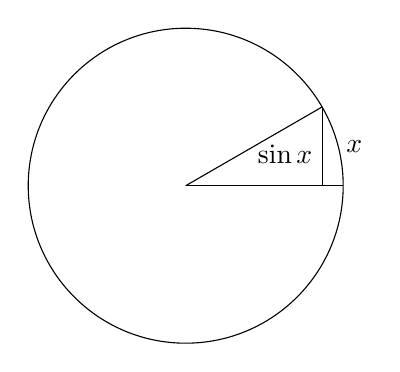
\begin{tikzpicture}[scale=2]
\draw (0,0) circle (1);
\draw (0,0) -- (1,0);
\draw (0,0) -- (0.866025404,0.5);
\draw (0.866025404,0.5) -- (0.866025404,0);
\node at (0.866025404,0.2) [anchor=east]{$\sin x$};
\node at (1.07,0.25) {$x$};
\end{tikzpicture}
\end{center}
\end{pro}

\begin{theo}[Cosine Limit]
When $x$ approaches $0,$
\[\frac{\cos x-1}{x}\]
approaches $0.$
\end{theo}

\begin{pro}
Refer to the same setup as above. Note that the altitude splits the radius into two pieces of length $\cos x$ and $1-\cos x.$ As $x$ approaches $0,$ the path $\sin x$ takes approaches the path $x$ takes, so the difference in the paths (i.e. $1-\cos x$) becomes negligible compared to $x.$
\end{pro}

\begin{theo}[Derivative of $\sin$]
The derivative of $f(x) = \sin x$ is $\cos x.$
\end{theo}

\begin{pro}
We use the limit definition of the derivative and the angle addition formulas.
\begin{align*}
\frac{d}{dx}\sin(x) &= \lim_{\Delta x \to 0} \frac{\sin(x+\Delta x) - \sin(x)}{\Delta x} \\
&= \lim_{\Delta x \to 0} \frac{\sin(x)\cos(\Delta x) + \sin(\Delta x)\cos(x) - \sin(x)}{\Delta x} \\
&= \lim_{\Delta x \to 0} \frac{\sin(x)(\cos(\Delta x) - 1) + \cos(x)\sin(\Delta x)}{\Delta x} \\
&= \lim_{\Delta x \to 0} \frac{\sin(x)(\cos(\Delta x) - 1)}{\Delta x} + \lim_{\Delta x \to 0} \frac{\cos(x)\sin(\Delta x)}{\Delta x} \\
&= \sin(x) \lim_{\Delta x \to 0} \frac{\cos(\Delta x) - 1}{\Delta x} + \cos(x) \lim_{\Delta x \to 0} \frac{\sin(\Delta x)}{\Delta x}
\end{align*}
Because $\lim\limits_{x\to 0}\frac{\sin x}{x}=1$ and $\lim\limits_{x\to 0}\frac{\cos x-1}{x}=0,$
\[\frac{d}{dx}\sin(x) = \cos(x).\]
\end{pro}

\begin{theo}[Derivative of $\cos$]
The derivative of $f(x) = \cos x$ is $-\sin x.$
\end{theo}

%\begin{pro}
%We use the limit definition of the derivative and the angle addition formulas.
%\begin{align*}
%\frac{d}{dx}\cos(x) &= \lim_{\Delta x \to 0} \frac{\cos(x+\Delta x) - \cos(x)}{\Delta x} \\
%&= \lim_{\Delta x \to 0} \frac{\cos(x)\cos(\Delta x) - \sin(x)\sin(\Delta x) - \cos(x)}{\Delta x} \\
%&= \lim_{\Delta x \to 0} \frac{\cos(x)(\cos(\Delta x) - 1) - \sin(x)\sin(\Delta x)}{\Delta x} \\
%&= \frac{d}{dx}\cos(x) = \cos(x) \lim_{\Delta x \to 0} \frac{\cos(\Delta x) - 1}{\Delta x} - \sin(x) \lim_{\Delta x \to 0} \frac{\sin(\Delta x)}{\Delta x}
%\end{align*}
%Because $\lim\limits_{x\to 0}\frac{\sin x}{x}=1$ and $\lim\limits_{x\to 0}\frac{\cos x-1}{x}=0,$
%\[\frac{d}{dx}\cos(x) = \cos(x)(0) - \sin(x)(1)\]
%\[\frac{d}{dx}\cos(x) = -\sin(x).\]
%\end{align*}
%\end{pro}

\begin{pro}
We just piggyback on the sin proof. Note that $\cos x=\sin(x+\frac{\pi}{2}),$ so the derivative of $\cos x$ is $\cos(x+\frac{\pi}{2})=\sin(x+\pi)=-\sin x.$
\end{pro}

A natural exercise comes from the following two theorems.

\begin{exer}[Periodic Derivatives]
If $f(x)=\sin x,$ find $f'(x),f''(x),f'''(x),$ and $f''''(x).$ Do the same for $f(x)=\cos x.$
\end{exer}

\begin{theo}[Derivative of $\tan$]
The derivative of $f(x) = \tan(x)$ is $\sec^2(x).$
\end{theo}

\begin{pro}
We just use the quotient rule. Note that
\begin{align*}
\frac{d}{dx}\tan(x) &= \frac{d}{dx}\left(\frac{\sin(x)}{\cos(x)}\right)\\
&= \frac{\cos(x)\cos(x) - \sin(x)(-\sin(x))}{\cos^2(x)} \\
&= \frac{\cos^2(x)+\sin^2(x)}{\cos^2(x)} \\
&= \frac{d}{dx}\tan(x) = \frac{1}{\cos^2(x)} \\
&= \frac{d}{dx}\tan(x) = \sec^2(x).
\end{align*}
\end{pro}

\begin{exer}[Derivatives of Reciprocal Functions]
Given how the trigonometric derivatives for sin, cos, and tan were derived, determine and prove the derivatives of csc, sec, and cot.
\end{exer}

\subsubsection{Optional: Taylor Series of $\sin$ and $\cos$}

This is officially optional, but I highly recommend you do it some time. It does not have to be on your first read-through of the handout, but you \textit{are} going to need to know this eventually.

With the derivatives of $\sin x$ and $\cos x$ in mind, it should be easy to express $f(x)=\sin x$ and $f(x)=\cos x$ as a Taylor Series. For people learning Calculus for the first time, this is optional but strongly recommended.

\begin{theo}[Maclaurin Series of $\sin$ and $\cos$]
The Maclaurin Series of $\sin \epsilon$ is $\sin\epsilon = \frac{\epsilon}{1!}-\frac{\epsilon^3}{3!}+\frac{\epsilon^5}{5!}-\cdots,$ and the Maclaurin Series of $\cos \epsilon$ is $\cos \epsilon = \frac{\epsilon^0}{0!}-\frac{\epsilon^2}{2!}+\frac{\epsilon^4}{4!}-\cdots.$
\end{theo}

\begin{pro}
If $f(x)=\sin x,$ note that
\begin{align*}
f(0+\epsilon)&=\frac{f(0)}{0!}+\frac{f'(0)\epsilon}{1!}+\frac{f''(0)\epsilon^2}{2!}+\frac{f'''(0)\epsilon^3}{3!}+\cdots \\
&=\frac{\sin 0}{0!}+\frac{\cos 0\epsilon}{1!}+\frac{-\sin 0\epsilon^2}{2!}+\frac{-\cos 0\epsilon^3}{3!}+\cdots \\
&=\frac{\epsilon}{1!}-\frac{\epsilon^3}{3!}+\frac{\epsilon^5}{5!}-\cdots.
\end{align*}
The proof for cosine follows nearly identically. (Do it on your own.)
\end{pro}

\begin{exer}
Find the Maclaurin Series of $x\cos x.$
\end{exer}

\subsection{Inverse of Trigonometric Functions}

We will implicitly differentiate here.

\begin{theo}[Arcsin Derivative]
The derivative of $f(x)=\arcsin(x)$ is $\frac{1}{\sqrt{1-x^2}}.$
\end{theo}

\begin{pro}
Let $f(x)=y$ and note that this implies $\sin y=x.$ Differentiating with respect to $x$ gives
\[\cos y\frac{dy}{dx}=1\]
\[\frac{dy}{dx}=\frac{1}{\cos y}\]
\[\frac{dy}{dx}=\frac{1}{\sqrt{1-x^2}}.\]
\end{pro}

\begin{theo}[Arccos Derivative]
The derivative of $f(x)=\arccos(x)$ is $-\frac{1}{\sqrt{1-x^2}}.$
\end{theo}

\begin{pro}
Let $f(x)=y$ and note that this implies $\cos y=x.$ Differentiating with respect to $x$ gives
\[-\sin y\frac{dy}{dx}=1\]
\[\frac{dy}{dx}=-\frac{1}{\sin y}\]
\[\frac{dy}{dx}=-\frac{1}{\sqrt{1-x^2}}.\]
\end{pro}

\begin{theo}[Arctan Derivative]
The derivative of $f(x)=\arctan(x)$ is $\frac{1}{1+x^2}.$
\end{theo}

\begin{pro}
Let $f(x)=y$ and note that this implies $\tan y=x.$ Differentiating with respect to $x$ gives
\[\sec^2y\frac{dy}{dx}=1\]
\[\frac{dy}{dx}=\frac{1}{\sec^2y}\]
\[\frac{dy}{dx}=\frac{1}{1+x^2}.\]
\end{pro}

The other three functions (the reciprocal functions) are left to the reader. You can either implicitly differentiate from the start or just use the quotient rule on $\sin,\cos,$ and $\tan$ -- both will work.

\begin{exer}[Derivative of Inverse of Reciprocal Trigonometric Functions]
Find the derivative of $\arccsc x,$ $\arcsec x,$ and $\arccot x.$
\end{exer}

\subsection{Exponential and Logarithmic Functions}
If this is your first time learning calculus, \href{https://www.geometryexplorer.xyz/pdfs/calc/e.pdf}{What is e?} is mandatory reading.

Here's a short summary of the facts about $e$ you should know.

\begin{theo}[Facts about e]
\hfill
\begin{enumerate}
\item $e$ is defined as the constant such that the derivative of $f(x)=e^x$ is $e^x.$
\item Furthermore, $k\cdot e^x$ is the \textbf{only class of functions with this property}, where $k$ is some arbitrary constant.
\item The Maclaurin Series of $e^x$ is \textbf{constructed} to allow this to happen.
\end{enumerate}
\end{theo}

Now we find and prove the derivative of $\ln x.$ It follows straight from the Inverse Function Rule, so try to do it on your own for a little bit.

\begin{theo}[Derivative of ln]
The derivative of $f(x)=\ln x$ is $\frac{1}{x}.$
\end{theo}

\begin{pro}
We put this straight into the Inverse Function Rule. Note that
\[(\ln x)'=\frac{1}{e^{\ln x}}\footnote{Remember that the derivative of $e^x$ is itself.}=\frac{1}{x},\]
as desired.
\end{pro}

\begin{exer}
Find the derivative of $f(x)=\log_a(g(x)).$
\end{exer}

\section{Examples}

Here are some worked examples from contests.

\begin{exam}[CHMMC 2021/4]
Let $P(x)=x^3-6x^2-5x+4.$ Suppose that $y$ and $z$ are real numbers such that
\[zP(y)=P(y-n)+P(y+n)\]
for all reals $n.$ Evaluate $P(y).$
\end{exam}

\begin{sol}
Note that this implies we want $P(y+n)-c$ to be an odd function about $n$ for some constant $c.$ Taking the derivative, we get
\[P'(y+n)=P'(y-n)\]
\[3(y+n)^2-12(y+n)-5=3(y-n)^2-12(y-n)-5\]
\[y^2+2yn+n^2-4y-4n=y^2-2yn+n^2-4y+4n\]
\[4yn-8n=0\]
\[y=2.\]
Thus the answer is $P(y)=2^3-6\cdot 2^2-5\cdot 2+4=8-24-10+4=\ansbold{-22}.$
\end{sol}

As a note, most contest problems are not going to require calculus -- there are other ways to do this. For instance, here you could just write everything in terms of $x-2$ to get the $x^2$ term to go away.

\pagebreak

\section{Problems}

Miscellaneous problems related to differentiation that are not on this handout will show up, such as limit problems and maximization/minimization problems.
\\

\noindent\minpt{32}

\psetquote{Violence is the last refuge of the incompetent.}{Foundation}

\begin{req}[]{2}
Prove that the derivative of $f(x)=e^{g(x)}$ is $e^{g(x)}g'(x).$
\end{req}

\begin{prob}[HMMT Calculus 2005/1]{2}
Let $f(x)=x^3+ax+b,$ with $a\neq b,$ and suppose that the tangent lines to the graph of $f$ at $x=a$ and $x=b$ are parallel. Find $f(1).$
\end{prob}

\begin{prob}[HMMT Calculus 2010/1]{2}
Suppose that $p(x)$ is a polynomial and that $p(x)-p'(x)=x^2+2x+1.$ Compute $p(5).$
\end{prob}

\begin{prob}[HMMT Calculus 2010/3]{3}
Let $p$ be a monic cubic polynomial such that $p(0)=1$ and such that all the zeroes of $p'(x)$ are also zeros of $p(x).$ Find $p.$ Note: monic means that the leading coefficient is $1.$
\end{prob}

\begin{req}[Two-Term AM-GM]{3}
Determine the minimum value $f(x)=x+\frac{1}{x}$ can take over positive $x.$
\end{req}

\begin{prob}[]{3}
Find the derivative of $\frac{4^x}{4^x+1}.$
\end{prob}

\begin{prob}[Dennis Chen]{3}
Find the equation of the line tangent to
\[\tan x+\sin x=y\cos x-1\]
at $(\frac{\pi}{4},2\sqrt{2}+1).$
\end{prob}

\begin{prob}[MIT OCW]{3}
Given that $f'(a)$ exists, show that $g(h) = \frac{f(a+h) - f(a)}{h}$ has a removable discontinuity at $h = 0$.
\end{prob}

\begin{prob}[HMMT Calculus 2007/2]{3}
Determine the real number $a$ having the property that $f(a)=a$ is a relative minimum of $f(x)=x^4-x^3-x^2+ax+1.$
\end{prob}

\begin{req}[HMMT Calculus 2006/2]{4}
Compute $\lim\limits_{x\to 0}\frac{e^{x\cos x}-1-x}{\sin(x^2)}.$
\end{req}

\begin{prob}[MAST Diagnostic 2020/C10]{4}
Find the maximum value of $k$ such that $(x+1)^4\geq kx^3$ for all $x.$
\end{prob}

\begin{prob}[Extension of C10]{2}
Find the range of values $k$ such that $(x+1)^4\geq kx^3$ for all $x.$
\end{prob}

\begin{prob}[AMC 12B 2020/22]{6}
What is the maximum value of $\frac{(2^t-3t)t}{4^t}$ for real values of $t?$
\end{prob}

\begin{req}[Leibniz Rule]{6}
Given two $n$th differentiable functions $f,g,$ prove that
\[(fg)^{(n)}(x)=\sum_{k=0}^{n}\binom{n}{k}f^{(k)}(x)g^{(n-k)}(x).\]
\end{req}

\begin{prob}[]{9}
The ellipse $\frac{x^2}{a^2}+\frac{y^2}{b^2}=1$ has a tangent $\ell$ that meets the $x$ and $y$ axes at $A$ and $B,$ respectively. If $O$ is the origin, find the minimal possible area of $\triangle AOB.$
\end{prob}

%\begin{prob}[Hong Kong TST 2021/1/1]{13}
%Find, \db{with proof}, all real triples $(a,b,c)$ satisfying
%\[(2^{2a}+1)(2^{2b}+2)(2^{2c}+8)=2^{a+b+c+5}.\]
%\end{prob}

\end{document}